\section{The Input-Length Variable and the Canvas Pareto}
\label{app:input_canvas}

\subsection{Input length: the second variable}

Equation~\ref{eq:dg} has two variables, and the second one matters more for
diffusion than for autoregression. Sweeping the prompt from roughly 1{,}000 to
6{,}800 tokens gives \arInputSlope\,ms per prompt token for the
autoregressive arm and \dgInputSlope\,ms for the diffusion arm ---
\inputSlopeRatio$\times$ steeper. The mechanism is direct: the autoregressive
model pays for the prompt once and every generated token then attends to a
cached KV, whereas each denoising step re-attends the full prompt, so prefill
is paid $K$ times.

\begin{figure}[h]
\centering
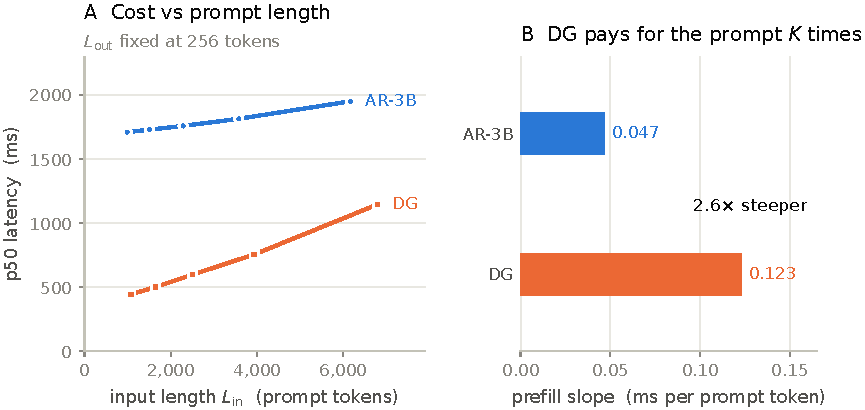
\includegraphics[width=\linewidth]{figures/fig3_input_sweep.pdf}
\caption{Input-length sweep at fixed $L_{\mathrm{out}}{=}\canvasLength$
(\artifact{results/issue44\_\{ar3b,dg\}\_input\_sweep.json}, BGL, $n{=}100$
per point). The prompt is lengthened by repeating the schema block, so the
task is unchanged. \textbf{B} is the finding: the diffusion model's prefill
slope is \inputSlopeRatio$\times$ the autoregressive model's.}
\label{fig:input}
\end{figure}

Every one-variable statement in this paper --- the crossover $L^{*}$, the
per-event ratios --- is calibrated at
the reference prompt of $\sim$\refPrompt\ tokens. At longer inputs the
diffusion base rises \inputSlopeRatio$\times$ faster and pushes $L^{*}$
upward. Extrapolated to a fixed $L_{\mathrm{out}}{=}\canvasLength$, the two
curves meet near $L_{\mathrm{in}} \approx 18{,}000$ tokens, beyond which the
autoregressive model is cheaper at \emph{any} output length. We did not
measure that far; the number is an extrapolation of two fitted slopes and is
quoted as an order of magnitude, not a boundary.

\subsection{A free Pareto improvement at canvas \texorpdfstring{$= 128$}{= 128}}

DiffusionGemma's canvas length is a configuration parameter, so we swept it.
At canvas $=128$ the base falls to \canvasOneTwentyEightBase\,ms ($-2.0\%$
relative to the canvas $=256$ measurement of \dgBase\,ms from
\artifact{results/issue44\_dg\_ksweep\_K8.json}; the canvas sweep's own
$L{=}256$ point measured 376.0\,ms in a separate run,
\artifact{results/issue66\_canvas\_256.json}, $n{=}200$) \emph{and} 9-field
F1 rises to \canvasOneTwentyEightFone\ --- an improvement on both axes
simultaneously.
At canvas $=64$ the base rises $48\%$, because the per-canvas fixed overhead
is paid twice as often; that setting is not viable. This is the only direct
experimental evidence that block size, not denoising schedule, is the
interesting design variable.

Neither canvas setting moves the per-event crossover. $L^{*}$ is set by the
prefill cost that dominates the base, and prefill does not shrink when the
canvas does. Tuning the canvas trades quality against step count; it does
not buy a different crossover.
